\documentclass{beamer}
\usepackage[utf8]{inputenc}

\usetheme{Madrid}
\usecolortheme{default}
\usepackage{amsmath,amssymb,amsfonts,amsthm}
\usepackage{txfonts}
\usepackage{tkz-euclide}
\usepackage{listings}
\usepackage{adjustbox}
\usepackage{array}
\usepackage{tabularx}
\usepackage{gvv}
\usepackage{lmodern}
\usepackage{circuitikz}
\usepackage{tikz}
\usepackage{graphicx}

\setbeamertemplate{page number in head/foot}[totalframenumber]

\usepackage{tcolorbox}
\tcbuselibrary{minted,breakable,xparse,skins}



\definecolor{bg}{gray}{0.95}
\DeclareTCBListing{mintedbox}{O{}m!O{}}{%
  breakable=true,
  listing engine=minted,
  listing only,
  minted language=#2,
  minted style=default,
  minted options={%
    linenos,
    gobble=0,
    breaklines=true,
    breakafter=,,
    fontsize=\small,
    numbersep=8pt,
    #1},
  boxsep=0pt,
  left skip=0pt,
  right skip=0pt,
  left=25pt,
  right=0pt,
  top=3pt,
  bottom=3pt,
  arc=5pt,
  leftrule=0pt,
  rightrule=0pt,
  bottomrule=2pt,
  toprule=2pt,
  colback=bg,
  colframe=orange!70,
  enhanced,
  overlay={%
    \begin{tcbclipinterior}
    \fill[orange!20!white] (frame.south west) rectangle ([xshift=20pt]frame.north west);
    \end{tcbclipinterior}},
  #3,
}
\lstset{
    language=C,
    basicstyle=\ttfamily\small,
    keywordstyle=\color{blue},
    stringstyle=\color{orange},
    commentstyle=\color{green!60!black},
    numbers=left,
    numberstyle=\tiny\color{gray},
    breaklines=true,
    showstringspaces=false,
}
%------------------------------------------------------------

\title
{11.2.9}
\date{September 25, 2025}
\author 
{AI25BTECH11003 - Bhavesh Gaikwad}



\begin{document}


\frame{\titlepage}
\begin{frame}{Question}
 AB is a line-segment. $\vec{P}$ and $\vec{Q}$ are points on opposite sides of AB such that each of them is equidistant from the points $\vec{A}$ and $\vec{B}$. Show that the line PQ is the perpendicular bisector of AB.
\end{frame}


\begin{frame}[fragile]
    \frametitle{Theoretical Solution}
Since $\vec{P}$ has the same distance from $\vec{A}$ and $\vec{B}$,
\begin{equation}
    \norm{\vec{P}-\vec{A}} = \norm{\vec{P}-\vec{B}}
\end{equation}

We know
\begin{equation}
 \norm{\vec{W}}^2 = {\vec{W}^\top\vec{W}}   
\end{equation}

Squaring both sides in Equation 1,
\begin{equation}
(\vec{P}-\vec{A})^\top(\vec{P}-\vec{A}) = (\vec{P}-\vec{B})^\top(\vec{P}-\vec{B})
\end{equation}

After Simplifing, we get
\begin{equation}
    \vec{P}^\top(\vec{B}-\vec{A}) = \dfrac{1}{2}(\, \norm{\vec{B}}^2 - \norm{\vec{A}}^2 \,)
\end{equation}

Similarly for $\vec{Q}$,
\begin{equation}
     \vec{Q}^\top(\vec{B}-\vec{A}) = \dfrac{1}{2}(\, \norm{\vec{B}}^2 - \norm{\vec{A}}^2 \,)
\end{equation}
\end{frame}


\begin{frame}[fragile]
    \frametitle{Theoretical Solution}
From A.5.1(Book),\\
The equation of perpendicular bisector of AB can be represented as
\begin{equation}
    \left( \vec{X} - \dfrac{\vec{A}+\vec{B}}{2} \right)^\top(\vec{B}-\vec{A}) = 0
\end{equation}


\begin{center}
    OR
\end{center}


\begin{equation}
    \vec{X}^\top(\vec{B}-\vec{A}) = \dfrac{1}{2}(\, \norm{\vec{B}}^2 - \norm{\vec{A}}^2 \,)
\end{equation}

\bigskip

A Point on line PQ can be represented as
\begin{equation}
    \vec{X} = \vec{P} + \lambda(\vec{P}-\vec{Q})
\end{equation}
\end{frame}

\begin{frame}[fragile]
    \frametitle{Theoretical Solution}
Taking dot production with $\vec{B} - \vec{A}$ on both sides,
\begin{equation}
    (\, \vec{B} - \vec{A} \,)^\top \vec{X} = (\, \vec{B} - \vec{A} \,)^\top \vec{P} + \lambda(\, \vec{B} - \vec{A} \,)^\top(\, \vec{P} - \vec{Q} \,)
\end{equation}
\begin{center}
    OR
\end{center}
\begin{equation}
    \vec{X}^\top(\, \vec{B} - \vec{A} \,) = \vec{P}^\top(\, \vec{B} - \vec{A} \,) + \lambda(\, \vec{P} - \vec{Q} \,)^\top(\, \vec{B} - \vec{A} \,)
\end{equation}

\begin{equation}
   \vec{X}^\top(\, \vec{B} - \vec{A} \,) = (1+\lambda)\vec{P}^\top(\, \vec{B} - \vec{A} \,) - \lambda\vec{Q}^\top(\, \vec{B} - \vec{A} \,)
\end{equation}


From Equation 4 and 5,
\begin{equation}
    \vec{X}^\top(\, \vec{B} - \vec{A} \,) = (1+\lambda)\left[\dfrac{1}{2}(\, \norm{\vec{B}}^2 - \norm{\vec{A}}^2 \,)\right]  - \lambda\left[\dfrac{1}{2}(\, \norm{\vec{B}}^2 - \norm{\vec{A}}^2 \,)\right]
\end{equation}

\begin{equation}
    \vec{X}^\top(\vec{B}-\vec{A}) = \dfrac{1}{2}(\, \norm{\vec{B}}^2 - \norm{\vec{A}}^2 \,)
\end{equation}

\bigskip

Since, Equation 7 and 13 are same.
\begin{align*}
    \boxed{\text{Hence Proved , Line PQ is a perpendicular bisector to line segment AB.}}
\end{align*}
\end{frame}

\begin{frame}[fragile]
    \frametitle{Example}
Assuming $\vec{A} = \myvec{1 \\ 0}$, $\vec{B} = \myvec{0 \\ 1}$, $\vec{P} = \myvec{0 \\ 0}$ and $\vec{Q} = \myvec{1 \\ 1}$

\begin{equation}
    \vec{B} - \vec{A} = \myvec{-1 \\ 1} \quad \& \quad \vec{P} - \vec{Q} = \myvec{-1 \\ -1} 
\end{equation}


\begin{equation}
    (\, \vec{B} - \vec{A} \,)^\top(\, \vec{P} - \vec{Q} \,) = 0
\end{equation}
Thus, Line PQ is perpendicular to line segment AB.\\\\

Let $\vec{M}$ be the midpoint of line segment AB.
\begin{equation}
    \vec{M} = \dfrac{\vec{A}+\vec{B}}{2} = \myvec{1/2 \\ 1/2}
\end{equation}
\end{frame}

\begin{frame}[fragile]
    \frametitle{Example}
Equation of line PQ,
\begin{equation}
    \vec{X} = \vec{P} + \lambda(\, \vec{P}-\vec{Q} \,)
\end{equation}

\begin{equation}
    \vec{X} = \lambda\myvec{-1 \\ -1}
\end{equation}

$\vec{M}$ satifies equation 18, thus Line PQ passes through midpoint of line segment AB. Thus PQ bisects AB.

\begin{align*}
\therefore \text{Line PQ is a perpendicular bisector to line segment AB.}
\end{align*}
\end{frame}


\begin{frame}{Image}
\begin{figure}
   \centering
    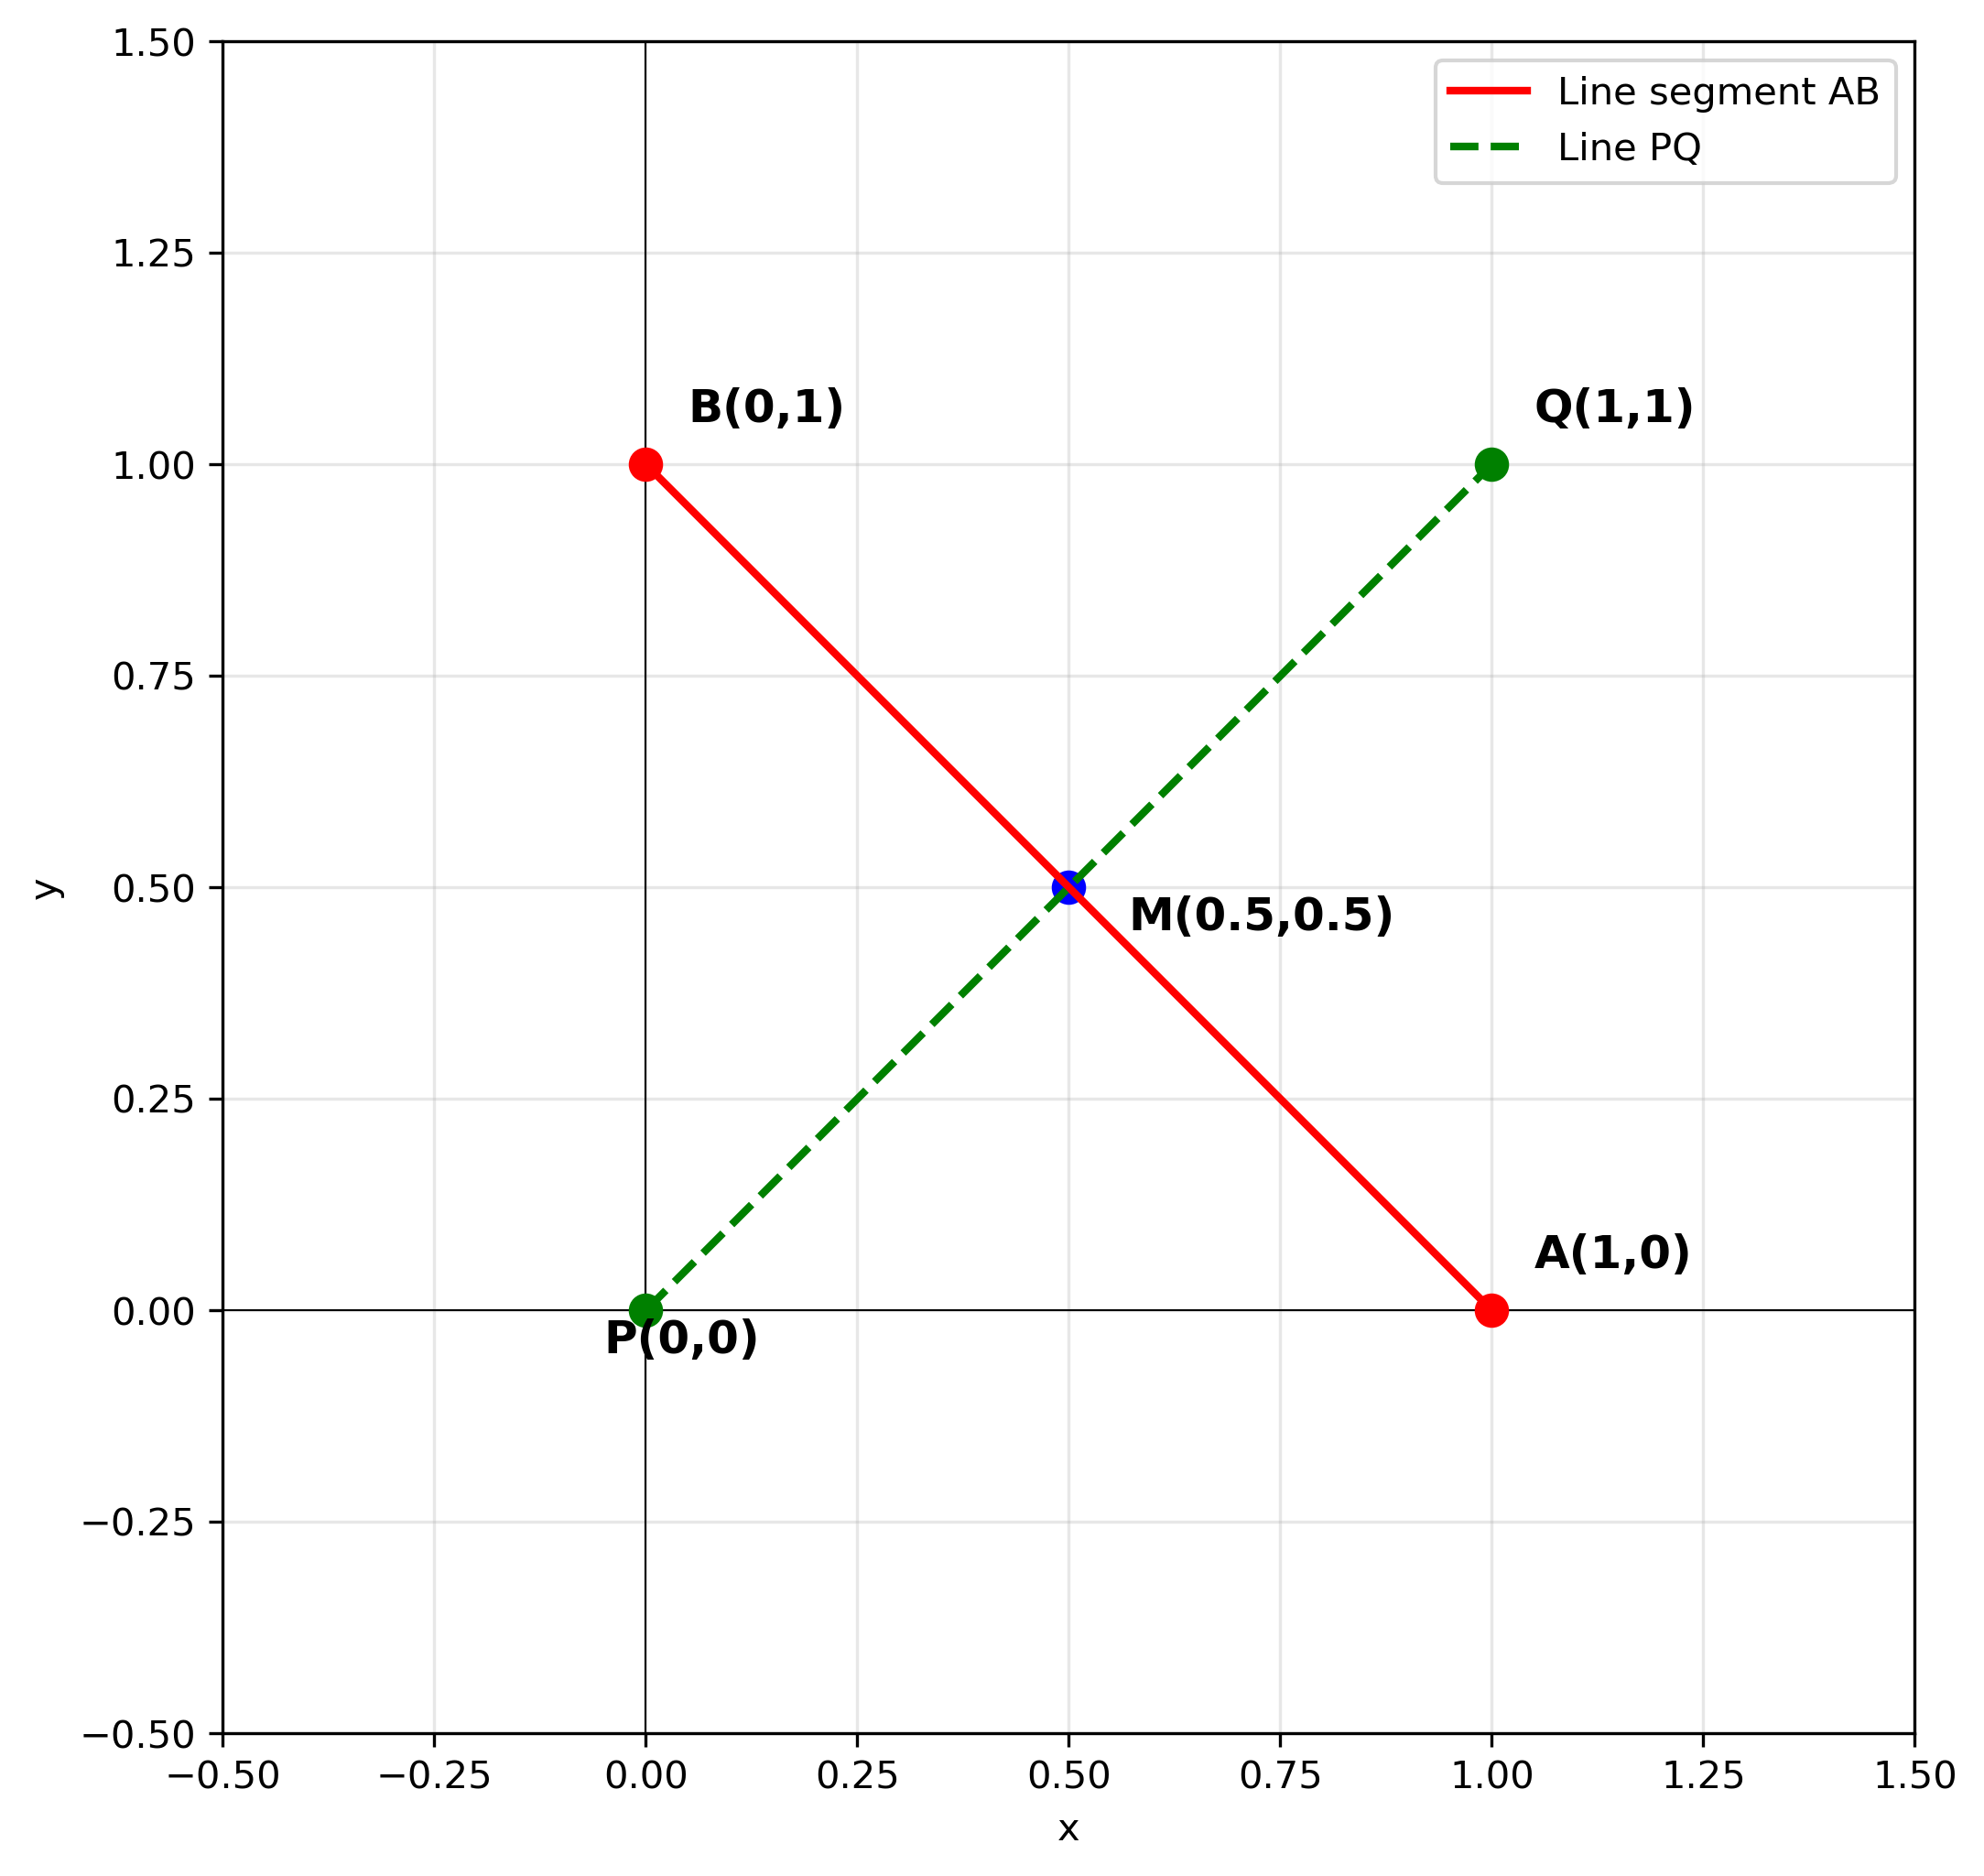
\includegraphics[width=\columnwidth, height=0.8\textheight, keepaspectratio]{figs/fig1.png}
    \label{fig:Beamer/figs/fig1.png}
\end{figure}
\end{frame}

\end{document}